%!TEX root = ../thesis.tex

\section{Introduction}
\paragraph{}
Creation of mesh in FEM can be expensive in terms of time and human resource.
One possible solution is trying to replace the geometric modelling tool in FEM by something more CAD-like.
NURBS, for example, is a standard mathematical model utilized in CAD industry.
Exact CAD geometric boundaries are achieved with the help of the NURBS curve.
This idea to be geometrically exact with a minimum discretization is adopted in Isogeometric analysis developed in 2005 \cite{Hug2005b} and further refined recently \cite{Zhang2007,Hug2005b,Cot2006,Cot2009,Baz2006a,Baz2006b}.
Furthermore, a simplified mesh refinement method by omitting the necessity for communication with the CAD geometry once the initial shape is received is also targeted \cite{Cot2007}.
% It shows advantage in the structure analysis (fig.~\ref{thinshell}) , fluid mechanics \citep{Buf2011} and dynamics (fig.~\ref{Femvsnurbs}).
The objectives of Isogeometric Analysis are to generalize the meshing process and improve the conventional Finite Element Analysis in the following ways \cite{Aur2010}.
\begin{enumerate}
    \item Offering remarkable degree of accuracy in representing complicated conformations and describing ordinary engineering moulds especially conic sections exactly.
    \item Minimizing geometrical errors and maintain high degree of accuracy in description of geometry at coarsest level of discretization
    \item Simplifying mesh refinement radically by omitting the necessity for communication with the CAD geometry
\end{enumerate}

\paragraph{}
Tensor product Non-Uniform Rational B-spline (NURBS) are well-known curve and surface representation method and have been adopted as a standard in computer graphics, computer-aided-design (CAD) \cite{Nas2003} and Initial Graphics Exchange Specification (IGES) standard since 1983 \cite{IGES1983}.
Nowadays, The employment of rational polynomial functions in description of geometry in CAD/CAM applications is becoming more and more extensive \cite{Pie1987}.
A general sculptured surface can be built easily with the help of NURBS \cite{Rog2001}.
One of its strongest reasons for that is its ability to represent conic curves and surface precisely.

\paragraph{}
The reason why the geometry is represented differently in computer aided design (CAD) and finite element analysis is because of different time they were born.
Commercial software with FEM has already been designed by the late 1960s and it spread to other engineering fields due to its convenience and accuracy.
It employs variational methods (the Calculus of variations) to minimize the error function in order to achieve a converge solution.
However, CAD, which gives an exact description on geometry, has not been developed until 1980s \cite{Dav2008}.
The first uni-graphics System (for 2D modelling and drafting) was sold by United Computing in 1975 \cite{Ste2010}.
Nowadays, CAD has been widespread and wins even more popularity than finite element analysis does. While, the geometric descriptions adopted by engineers today for CAD and analysis are totally different.
One rough estimate \cite{Hug2005} suggests that more than half of the overall analysis time is spent on meshing in the industries such as automotive and aerospace where complex shapes are involved.
Furthermore, frequent design modifications in fast pace, modern society restricts the usage of analysis if a new mesh cannot be created in a short duration.

\paragraph{}
In current Isogeometric analysis, accuracy problems with numerical integration of a rational polynomials attract significant attention \cite{Hug2010,Sev2011,Aur2012}.
Furthermore, incapability to create a set of control points to fit an inhomogeneous essential boundary condition may lead to considerable errors and lower converge speed due to the non-interpolatory characteristics of the NURBS surface and curves \cite{Wang2010,Wol2011,Koo2013}.
Besides, although numerous amount of research has been conducted on improving the algorithm efficiency \cite{Boo1972,Qin1996,Cho1990,Gra1992,Pan2001,Wang2012}, most of the time is devoted to calculate the basis function which restricts the usage of high order basis function in 3D problems.
Moreover, one of the most critical problems in the existing Isogeometric analysis lies in dimension incompatibility.
It is based on FEM where 3D NURBS solids are required for meshing in 3D problems but only the boundary is described in CAD system.
Further meshing process for converting input surface data to higher dimension physical geometry in isogeometric analysis has been referred to as ``analysis-aware modelling'' \cite{Coh2010}.
Considerable research on solving this incompatibility by domain parameterization has been performed on using a variety of methods \cite{Yang2007,Aig2009,Mar2009,Qian2011}.

\paragraph{}
In order to eliminate the need for domain parameterization, a NURBS based Boundary Element Method (BEM) is proposed \cite{Li2011,Taka2012,Beli2013,Sco2013,Sim2013}.
In BEM, only the boundary was discretised, contributing to a reduction of the spatial dimension by one and hence be fully compatible with CAD output geometric data.
Moreover, error induced in boundary condition fitting and numerical integration decreases and higher order basis function can be utilized to achieve higher accuracy.
Nevertheless, the fundamental solution satisfying the governing differential equations in the domain must be available.
Unfortunately, this fundamental solution may be extremely complex.

\paragraph{}
A Scaled Boundary finite element method (SBFEM) which has similarity with both the FEM and the BEM is proposed to eradicate the necessity of fundamental solution in BEM. SBFEM is a novel semi-analytical approach developed by Wolf and Song \cite{Wol1999}.
As a method developed based on FEM and BEM, SBFEM is a fundamental-solution-less boundary element method which keeps the benefits of the both as well as provides some effective solutions to the limitations to the FEM and the BEM \cite{Wol1999}.
The fundamental solution is no longer required, spatial dimension is reduced by one as only the boundary is meshed with surface elements which lead to decline in the number of unknowns and achievement of infinite boundary \cite{Wol2003}.

\paragraph{}
In this chapter,the idea of isogeometric analysis \cite{Hug2005}, NURBS and IGES will first be introduced.
After that, computational mechanics method including FEM, BEM and SBFEM will be discussed.
Furthermore, data mining technology will be introduced in order to perform an adaptive analysis.
Finally, STL file will be discussed to extend the proposed method to 3D problems.

% \section{Computational mechanics in civil engineering}

%     \subsection{Mathematical model in engineering mechanics}

%     \subsection{Numerical methods}

%     \subsection{Computational mechanics in modern age}

% \section{Current challenges in numerical analysis}

%     \subsection{Human effort on mesh generation}

%     \subsection{Imperfection in geometric representation}

%     \subsection{Lack of re-meshing scheme}

% \section{Proposed approach}
% \paragraph{}


% \section{Research contribution}

%     \subsection{Meshing based on CAD output in 2D and 3D}

%     \subsection{High quality elements by Quad-tree}

%     \subsection{Auto re-meshing based on error}

% \section{Objectives and scope}

% \section{Organization of the thesis}

% \section{List of publications}


    % /* cspell:disable */
    % \begin{figure}[h!]
    %     \scalebox{1}{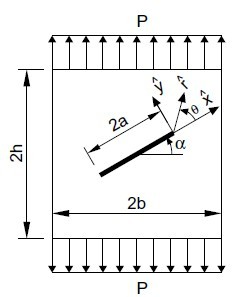
\includegraphics{chapter1/img/crackproblem.jpg}}
    % \end{figure}
    % /* cspell:enabled*/
